\documentclass[11pt,a4paper]{article}

\usepackage[utf8]{inputenc}
\usepackage[T1]{fontenc}
\usepackage{lmodern}
\usepackage[margin=1in]{geometry}
\usepackage{amsmath,amssymb,amsfonts,amsthm}
\usepackage{mathtools}
\usepackage{booktabs}
\usepackage{tabularx}
\usepackage{array}
\usepackage{xcolor}
\usepackage{enumitem}
\usepackage{parskip}
\usepackage{microtype}
\usepackage{tikz}
\usetikzlibrary{arrows.meta,positioning}
\usepackage[most]{tcolorbox}
\usepackage{hyperref}

\setlength{\emergencystretch}{1.5em}

\hypersetup{
    colorlinks=true,
    linkcolor=blue!60!black,
    urlcolor=blue!60!black,
    citecolor=blue!60!black,
    pdftitle={A Calculus-Based Primer on Riemannian Manifold Steering},
    pdfauthor={Frank W. Elliott Jr.}
}

\newcolumntype{Y}{>{\raggedright\arraybackslash}X}
\newcommand{\R}{\mathbb{R}}
\newcommand{\DKL}{D_{\mathrm{KL}}}
\DeclareMathOperator{\diag}{diag}
\DeclareMathOperator{\Exp}{Exp}
\DeclareMathOperator{\Log}{Log}
\DeclareMathOperator{\erf}{erf}

\theoremstyle{definition}
\newtheorem{definition}{Definition}[section]
\newtheorem{remark}{Remark}[section]

\newtcolorbox{keyidea}[1][]{
    enhanced,
    breakable,
    colback=blue!4!white,
    colframe=blue!55!black,
    fonttitle=\bfseries,
    boxrule=0.6pt,
    arc=2pt,
    left=8pt,
    right=8pt,
    top=6pt,
    bottom=6pt,
    title={#1}
}

\title{\textbf{A Calculus-Based Primer on Riemannian Manifold Steering}\\[0.4em]
\large From Multivariable Calculus and ODEs to Neural Geodesics}
\author{}
\date{November 11, 2026}

\begin{document}

\maketitle

\begin{abstract}
\noindent
\textbf{Prerequisite level:} Four semesters of undergraduate calculus---single-variable derivatives and integrals (Calculus~I--II), multivariable and vector calculus with Jacobians and parameterized surfaces (Calculus~III), and ordinary differential equations with initial/boundary value problems and introductory matrix algebra (Calculus~IV). Starting from real-world engineering and scientific applications, this primer defines the geometric vocabulary of \textbf{Riemannian manifold steering}, builds concrete visual intuition for why straight-line activation interventions break down in nonlinear neural networks, derives pullback metrics and the Levi-Civita geodesic ODE directly from the multivariable chain rule, connects numerical BVP/IVP solvers to smooth activation functions, and provides clickable references to both the literature and the accompanying workspace implementation.
\end{abstract}

\tableofcontents

\vspace{0.75em}
\hrule
\vspace{0.75em}

% =============================================================================
\section{Why Care? Practical Applications of Manifold Steering}
\label{sec:applications}
% =============================================================================

Modern AI systems---from Large Language Models (LLMs) and reasoning models to protein generators and robot controllers---store rich internal knowledge inside high-dimensional hidden layers. Yet retraining or fine-tuning billions of weights every time we want to adjust safety boundaries, reasoning depth, tone, or physical constraints is slow, expensive, and prone to catastrophic forgetting.

\textbf{Inference-time steering} offers an attractive alternative: nudge the model's internal activations \emph{on the fly} during a forward pass, with zero weight updates. However, naive straight-line vector addition ($h + \alpha v$) treats neural activation space as flat Euclidean $\R^D$. Push $\alpha$ slightly too far and the activation vector leaves the narrow curved surface (\emph{manifold}) of valid representations that the network learned during training---causing garbled text, degraded reasoning, or physically impossible outputs.

\textbf{Riemannian manifold steering} keeps interventions \emph{on the manifold} by following curved shortest paths (\textbf{geodesics}) measured with the network's own derivatives. Across industry and science, this unlocks six high-impact applications (summarized in Table~\ref{tab:applications}):

\begin{enumerate}[leftmargin=*]
    \item \textbf{Test-Time LLM Safety \& Alignment Without the ``Alignment Tax'':}
    Fine-tuning LLMs for safety or policy compliance often incurs an \emph{alignment tax}---blunting coding, math, or creative capabilities---while linear steering vectors degrade fluency at strong intervention scales. Steering along on-manifold geodesics lets practitioners dial behavioral traits (honesty, refusal boundaries, formality, domain persona) smoothly at inference time while keeping hidden states inside high-fluency regions, preserving downstream benchmark utility without retraining~\cite{wurgaft2026manifold,oozeer2026riemannian}.

    \item \textbf{Faithful Chain-of-Thought \& Curing ``Overthinking'' in Reasoning Models:}
    Large Reasoning Models (such as DeepSeek-R1 and o1-class models) face two acute inference-time failure modes: logical drift across multi-step proofs, and \emph{overthinking}---endless self-doubt and redundant verification loops that burn $3\times$--$5\times$ extra compute and latency. Subtracting a single Euclidean vector hits a hard accuracy ceiling because off-manifold noise corrupts intermediate logic. Manifold-guided steering (\emph{GeoSteer}~\cite{kazama2026geosteer} and low-dimensional manifold projection~\cite{huang2025overthinking}) guides reasoning trajectories along valid logical states, cutting output token counts by \textbf{up to $71\%$} on math, code, and QA benchmarks while maintaining or improving accuracy.

    \item \textbf{Controlling Cyclical, Ordered, and Multi-Dimensional Concepts:}
    Many real-world concepts inside neural networks are \emph{provably non-linear}: calendar dates and months, clock angles, spatial 3D orientations, and ordered severity scales live on closed loops, tori, or curved surfaces rather than straight lines~\cite{engels2024nonlinear}. A straight Euclidean chord between two points on a circle cuts straight across the empty interior! Riemannian geodesics travel naturally \emph{around} the curved concept manifold, enabling consistent multi-step and cyclic control without prompt-level supervision~\cite{oozeer2026riemannian}.

    \item \textbf{Actionable Counterfactual Explanations in Medical \& High-Stakes AI:}
    When a clinical classifier flags a radiology scan or a financial model denies an application, experts ask a counterfactual question: \emph{``What is the smallest realistic change to this input that flips the model's decision?''} Standard Euclidean optimization ($\min_{\delta x}\|\delta x\|_2$) produces adversarial static or anatomically impossible ``ghost'' organs---just like averaging a \texttt{`4'} and a \texttt{`9'} in pixel space creates a double-exposed ghost digit. Boundary-value geodesics under a pullback metric traverse plausible, on-manifold morphology, giving clinicians and auditors trustworthy glass-box explanations~\cite{arvanitidis2018oddity,wurgaft2026manifold}.

    \item \textbf{Protein Engineering, Directed Evolution \& Drug Discovery:}
    Generative latent-variable models compress discrete protein sequences and molecular structures into continuous spaces to design novel therapeutics and enzymes. Linearly interpolating between two functional proteins slices through ``dead zones'' of unfolded, non-viable sequences. Equipping the latent space with a decoder pullback metric turns geodesics into biologically meaningful mutational pathways that preserve structural stability and evolutionary plausibility from start to target~\cite{detlefsen2022protein}.

    \item \textbf{Artifact-Free Generative Media \& Safe Robotic Motion Planning:}
    In image, video, and audio synthesis, geodesic latent interpolation eliminates off-manifold ``ghosting'' and abrupt perceptual jumps~\cite{arvanitidis2018oddity,hauberg2019onlybayes}. In robotics, learning a Riemannian skill manifold from human demonstrations allows a robot arm to plan smooth, collision-free trajectories as geodesics: obstacles dynamically inflate the local metric tensor $g(u)$ so minimum-energy paths curve safely around hazards while staying within physically feasible joint configurations~\cite{beikmohammadi2021robotics}.
\end{enumerate}

\begin{table}[ht!]
\centering
\footnotesize
\renewcommand{\arraystretch}{1.32}
\begin{tabularx}{\textwidth}{@{} >{\bfseries\raggedright\arraybackslash}p{0.23\textwidth} >{\raggedright\arraybackslash}p{0.35\textwidth} Y @{}}
\toprule
Application Domain & \textbf{Failure of Linear / Euclidean Approach} & \textbf{What Geodesic Manifold Steering Achieves} \\
\midrule
LLM Alignment \& Safety & Off-manifold drift degrades fluency and reasoning at strong steering scales. & Smooth, training-free control of safety, honesty, and persona without utility loss~\cite{wurgaft2026manifold,oozeer2026riemannian}. \\
\addlinespace
Chain-of-Thought Reasoning & High-dimensional noise breaks multi-step logic; overthinking wastes tokens. & Preserves step-by-step faithfulness~\cite{kazama2026geosteer} and cuts overthinking tokens by up to $71\%$~\cite{huang2025overthinking}. \\
\addlinespace
Cyclic \& Curved Concepts & Chords cut through invalid interiors of circular/curved features (dates, pose). & Follows intrinsic curved geometry cleanly across sequential or periodic states~\cite{engels2024nonlinear,oozeer2026riemannian}. \\
\addlinespace
High-Stakes Auditing & Minimum-$L_2$ perturbations yield adversarial static or ghosted superpositions. & Plausible, on-manifold counterfactual trajectories for medical and safety review~\cite{arvanitidis2018oddity}. \\
\addlinespace
Protein \& Drug Design & Linear latent mixes pass through unfolded, non-functional ``dead zones.'' & Biologically viable mutational paths that respect structural \& evolutionary constraints~\cite{detlefsen2022protein}. \\
\addlinespace
Robotics \& Media Synthesis & Ghosted visual morphs; latent robot paths cut into obstacles or joint locks. & Smooth perceptual transitions and obstacle-avoiding geodesic motion skills~\cite{beikmohammadi2021robotics}. \\
\bottomrule
\end{tabularx}
\caption{Practical domains where Riemannian manifold steering overcomes flat Euclidean interventions.}
\label{tab:applications}
\end{table}

\begin{keyidea}[The Open Secret of Differential Geometry]
You do \emph{not} need years of abstract topology to understand or build manifold steering. Almost every intimidating term in Riemannian geometry---\emph{manifold, coordinate chart, tangent space, pushforward, pullback metric, volume form, geodesic, Christoffel symbol}---is a systematic reorganization of tools you already know from \textbf{Calculus~II--IV}: parametric arc-length integrals, the multivariable chain rule, Gauss's surface-area formula, quadratic Taylor approximations, and systems of second-order ODEs.
\end{keyidea}

% =============================================================================
\section{Your Calculus I--IV Toolkit}
\label{sec:calculus-toolkit}
% =============================================================================

Before introducing differential-geometric terminology, Table~\ref{tab:calc-bridge} maps familiar undergraduate calculus tools directly onto the objects used in manifold steering.

\begin{table}[ht!]
\centering
\small
\renewcommand{\arraystretch}{1.35}
\begin{tabularx}{\textwidth}{@{} l >{\raggedright\arraybackslash}p{0.23\textwidth} >{\raggedright\arraybackslash}p{0.26\textwidth} Y @{}}
\toprule
\textbf{Course} & \textbf{Calculus Tool} & \textbf{Familiar Formula} & \textbf{Role in Manifold Steering} \\
\midrule
\textbf{Calc I} & Smoothness \& $2$nd derivative & $f \in C^2 \implies f''(x)$ continuous & Why smooth activations (\texttt{SMU}~\cite{biswas2022smu}, \texttt{Softplus}) have smooth curvature while \texttt{ReLU} concentrates curvature into sharp kinks. \\
\addlinespace
\textbf{Calc II} & Parametric arc length \& Taylor series & $L = \int_0^1 \|\vec{r}\,'(t)\|_2\,dt$ & Measuring true representational or KL-divergence distance along a steering curve. \\
\addlinespace
\textbf{Calc III} & Parameterized surface \& Chain Rule & $\frac{d}{dt}h(\gamma(t)) = J_h(\gamma(t))\,\dot{\gamma}(t)$ & Turning a chart velocity $\dot{\gamma}(t)$ into a neuron-space velocity via the Jacobian matrix $J_h$. \\
\addlinespace
\textbf{Calc III} & Surface-area magnification & $dA = \sqrt{EG - F^2}\,du^1 du^2$ & The \textbf{Riemannian volume element} $\sqrt{\det g(u)}$, highlighting steep ``semantic cliffs.'' \\
\addlinespace
\textbf{Calc IV} & $2$nd-order ODEs (IVP vs.\ BVP) & $\ddot{u} = F(u, \dot{u})$ & Computing \textbf{geodesics} either between two fixed endpoints (BVP) or along an initial concept velocity (IVP). \\
\bottomrule
\end{tabularx}
\caption{Correspondence between four-semester undergraduate calculus and Riemannian manifold steering.}
\label{tab:calc-bridge}
\end{table}

% =============================================================================
\section{Geometric Intuition: What Is ``Steering,'' and Why Do Straight Lines Fail?}
\label{sec:motivation}
% =============================================================================

\subsection{Linear Activation Steering}

When a trained neural network processes an input $x$ (such as a $28 \times 28$ handwritten digit or a language-model token sequence), each hidden layer $\ell$ produces an \textbf{activation vector} $h \in \R^D$---a list of $D$ real numbers encoding what the model currently represents.

\textbf{Activation steering} intervenes on $h$ \emph{at inference time} (without changing model weights) to guide behavior smoothly from a source concept $A$ toward a target concept $B$:
\begin{itemize}[leftmargin=*]
    \item In Large Language Models (LLMs), $A$ might represent \emph{sycophantic agreement} and $B$ \emph{objective candor}~\cite{turner2023actadd,zou2023repe,rimsky2024caa}.
    \item In our interactive MNIST notebook (\href{run:../notebooks/manifold_steering_demo.py}{\texttt{notebooks/manifold\_steering\_demo.py}}), $A$ is a validation digit \texttt{`4'} ($x_A$) and $B$ is a validation digit \texttt{`9'} ($x_B$).
\end{itemize}

Standard \textbf{linear steering} (\emph{Activation Addition} / \emph{Contrastive Activation Addition}) forms the difference vector $v = h_B - h_A$ and translates along a \textbf{straight Euclidean line}:
\begin{equation}
    h_{\mathrm{lin}}(t) = h_A + t\,(h_B - h_A) = (1 - t)\,h_A + t\,h_B, \qquad t \in [0, 1].
    \label{eq:linear-steering}
\end{equation}
Equation~\eqref{eq:linear-steering} implicitly assumes the \textbf{Linear Representation Hypothesis (LRH)}~\cite{park2024linear}: that semantic features live in a flat Euclidean space where equal vector increments yield uniform, valid changes in meaning everywhere.

\subsection{Three Geometric Failure Modes of Straight Lines}

Drawing a straight ruler line on a flat Mercator world map from Tokyo to Paris looks short on paper, yet on the curved Earth it detours thousands of kilometers away from the true great-circle flight path. In nonlinear neural networks, straight Euclidean lines fail in three analogous ways:

\begin{enumerate}[leftmargin=*]
    \item \textbf{Off-Manifold ``Ghosting'':} Halfway along the straight chord between a \texttt{`4'} and a \texttt{`9'} ($t = 0.5$), the average $\frac{1}{2}x_A + \frac{1}{2}x_B$ superimposes two faint ghost digits instead of morphing the open top strokes of the \texttt{`4'} into the closed loop of a \texttt{`9'}. In LLMs, off-manifold hidden states produce incoherent text or sudden capability collapse~\cite{wurgaft2026manifold,oozeer2026riemannian}.
    \item \textbf{Plateaus and Semantic Cliffs (Non-Uniform Speed):} Deep inside the \texttt{`4'} decision basin, advancing $t$ from $0.00$ to $0.40$ barely alters the output probabilities ($p(\text{\texttt{`4'}}) \approx 0.999$). Then, between $t = 0.48$ and $t = 0.52$, the straight line slices across a narrow \textbf{decision boundary} where class probabilities flip abruptly and Shannon entropy spikes. A Euclidean ruler assigns both intervals length $0.04$, completely blind to how fast the network's output is changing.
    \item \textbf{Curved Representation Surfaces:} Nonlinear layers (convolutions, attention routing, gated MLPs) bend low-dimensional input variations into curved surfaces inside downstream activation spaces~\cite{arvanitidis2018oddity,engels2024nonlinear}.
\end{enumerate}

\textbf{Manifold steering}~\cite{wurgaft2026manifold,oozeer2026riemannian,kazama2026geosteer} resolves these failures by equipping our coordinates with a \textbf{position-dependent local ruler}---the \textbf{pullback Riemannian metric} $g(u)$ computed from the network's own derivatives---and steering along \textbf{geodesics}: curves of minimum path energy and constant semantic speed (Figure~\ref{fig:pipeline}).

\begin{figure}[ht!]
\centering
\resizebox{\textwidth}{!}{%
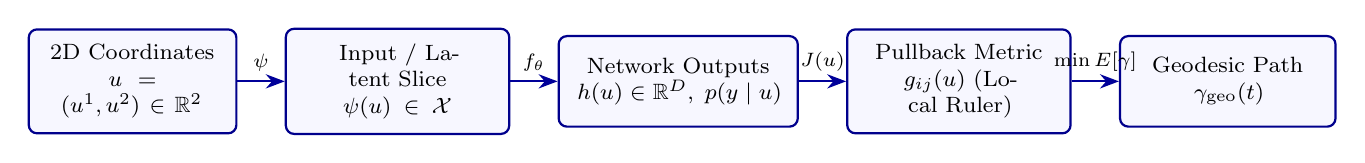
\begin{tikzpicture}[
    node distance=0.6cm,
    box/.style={
        draw=blue!55!black,
        fill=blue!3!white,
        rounded corners=3pt,
        thick,
        align=center,
        font=\footnotesize,
        inner sep=5.5pt,
        minimum height=1.15cm
    },
    arr/.style={-{Stealth[length=2.4mm,width=1.8mm]}, thick, draw=blue!60!black}
]
\node[box, text width=2.25cm] (u) {2D Coordinates\\$u = (u^1, u^2) \in \R^2$};
\node[box, text width=2.45cm, right=of u] (x) {Input / Latent Slice\\$\psi(u) \in \mathcal{X}$};
\node[box, text width=2.65cm, right=of x] (h) {Network Outputs\\$h(u) \in \R^D,\; p(y\mid u)$};
\node[box, text width=2.45cm, right=of h] (g) {Pullback Metric\\$g_{ij}(u)$ (Local Ruler)};
\node[box, text width=2.35cm, right=of g] (geo) {Geodesic Path\\$\gamma_{\mathrm{geo}}(t)$};

\draw[arr] (u) -- node[above, font=\scriptsize] {$\psi$} (x);
\draw[arr] (x) -- node[above, font=\scriptsize] {$f_\theta$} (h);
\draw[arr] (h) -- node[above, font=\scriptsize] {$J(u)$} (g);
\draw[arr] (g) -- node[above, font=\scriptsize] {$\min E[\gamma]$} (geo);
\end{tikzpicture}%
}
\caption{End-to-end pipeline of Riemannian manifold steering.}
\label{fig:pipeline}
\end{figure}

% =============================================================================
\section{Core Vocabulary: From Calc III Surfaces to Manifolds}
\label{sec:vocabulary}
% =============================================================================

Let us define each geometric object by translating it directly into Calculus~III.

\begin{definition}[Smooth Manifold $M$]
An $m$-dimensional \textbf{smooth manifold} $M$ is a space that may curve or close up globally (such as the unit sphere $S^2 \subset \R^3$), but around every point $p \in M$, a sufficiently small neighborhood can be smoothly and invertibly flattened onto an open subset of ordinary Euclidean space $\R^m$~\cite{morgan2016riemannian,boumal2023intro}.
\end{definition}

\noindent
\textbf{Calculus III translation:} Every smooth 2D parameterized surface $\vec{r}(u^1, u^2)$ in $\R^3$ without self-intersections or sharp creases is a 2D manifold ($m = 2$). In neural networks, we simply replace $\R^3$ with the $D$-dimensional activation space $\R^D$ (where $D$ may be $128$, $784$, or $4096$). For an interactive 3D sphere-chart warm-up, see \href{run:notebooks/manifold_atlas.py}{\texttt{theory/notebooks/manifold\_atlas.py}}.

\begin{definition}[Coordinate Chart $\varphi$ and Parameterization $\psi = \varphi^{-1}$]
A \textbf{coordinate chart} $\varphi$ assigns flat coordinates $u = (u^1, \dots, u^m) \in U \subseteq \R^m$ to a patch of the manifold. Its inverse map $\psi = \varphi^{-1} : U \to \mathcal{X}$ (\textbf{parameterization}) maps flat coordinates $u$ into the ambient space $\mathcal{X}$. A collection of overlapping charts covering $M$ is called a \textbf{smooth atlas}.
\end{definition}

\noindent
\textbf{How Stage~1 constructs an isometric 2D chart:} Given three anchor digits $(x_A, x_B, x_C)$ in $784$-dimensional image space ($28 \times 28 = 784$), \texttt{TangentChart2D.from\_three\_images} in \href{run:../src/models/MNIST/steering.py}{\texttt{src/models/MNIST/steering.py}} applies \textbf{Gram--Schmidt orthonormalization} to build two unit, mutually perpendicular basis images $e_1, e_2 \in \R^{1 \times 28 \times 28}$:
\begin{equation}
    e_1 = \frac{x_B - x_A}{\|x_B - x_A\|_2}, \qquad
    \tilde{e}_2 = (x_C - x_A) - \langle x_C - x_A, e_1 \rangle\, e_1, \qquad
    e_2 = \frac{\tilde{e}_2}{\|\tilde{e}_2\|_2},
    \label{eq:gram-schmidt}
\end{equation}
and decodes any 2D coordinate pair $u = (u^1, u^2) \in \R^2$ via the affine plane
\begin{equation}
    \psi(u^1, u^2) = x_0 + u^1 e_1 + u^2 e_2.
    \label{eq:chart-decode}
\end{equation}
\emph{Why orthonormality matters:} Because $\|e_1\|_2 = \|e_2\|_2 = 1$ and $\langle e_1, e_2 \rangle = 0$, the Pythagorean theorem guarantees
\[
    \|\psi(u) - \psi(v)\|_2^2 = \|(u^1 - v^1)e_1 + (u^2 - v^2)e_2\|_2^2 = (u^1 - v^1)^2 + (u^2 - v^2)^2 = \|u - v\|_2^2.
\]
Thus our 2D screen coordinates $(u^1, u^2)$ introduce \textbf{zero chart distortion} (an \emph{isometry} into pixel space): every curved decision boundary and metric ridge originates $100\%$ from the neural network.

\begin{definition}[Immersion $h$, Tangent Space $T_{h(u)}M$, and Pushforward / Jacobian $J_h$]
Feed the decoded input $\psi(u)$ into a smooth hidden layer $f_\ell : \mathcal{X} \to \R^D$, defining the composite map
\[
    h(u) \coloneqq f_\ell\bigl(\psi(u)\bigr) \in \R^D.
\]
Suppose $\gamma(t) = \bigl(u^1(t), \dots, u^m(t)\bigr)$ is a smooth curve in chart coordinates for $t \in [0, 1]$ with velocity $\dot{\gamma}(t) = \bigl(\dot{u}^1(t), \dots, \dot{u}^m(t)\bigr)$. By the \textbf{Calculus~III Multivariable Chain Rule}, the curve's velocity inside $\R^D$ is
\begin{equation}
    \frac{d}{dt} h\bigl(\gamma(t)\bigr) = \sum_{i=1}^m \frac{\partial h}{\partial u^i}\,\dot{u}^i(t) = J_h\bigl(\gamma(t)\bigr)\,\dot{\gamma}(t),
    \label{eq:chain-rule}
\end{equation}
where $J_h(u) \in \R^{D \times m}$ is the \textbf{Jacobian matrix} whose columns are the partial derivative vectors $\partial_i h(u) = \frac{\partial h}{\partial u^i} \in \R^D$:
\[
    J_h(u) = \begin{bmatrix} \vert & & \vert \\ \partial_1 h(u) & \cdots & \partial_m h(u) \\ \vert & & \vert \end{bmatrix}.
\]
When $J_h(u)$ has full column rank $m$, $h$ is called an \textbf{immersion}. As $\dot{\gamma}$ ranges over $\R^m$, the output velocities $J_h(u)\,\dot{\gamma}$ span an $m$-dimensional flat plane in $\R^D$ tangent to the surface at $h(u)$, called the \textbf{tangent space} $T_{h(u)}M$. Multiplying a chart vector $\dot{\gamma}$ by $J_h(u)$ is called the \textbf{pushforward} (or differential $dh_u$).
\end{definition}

% =============================================================================
\section{The Local Ruler: Pullback Riemannian Metrics (\texorpdfstring{$g_{ij}$}{g\_ij})}
\label{sec:pullback-metrics}
% =============================================================================

\subsection{Deriving the Pullback Metric from Calculus II Arc Length}

In Calculus~II, the arc length of the neuron-space trajectory $t \mapsto h(\gamma(t)) \in \R^D$ is the integral of its Euclidean speed:
\[
    L[\gamma] = \int_0^1 \left\| \frac{d}{dt} h\bigl(\gamma(t)\bigr) \right\|_2 dt.
\]
Substitute the Chain Rule~\eqref{eq:chain-rule} into the squared norm $\|w\|_2^2 = w^\top w$:
\begin{equation}
    \left\| \frac{d}{dt} h\bigl(\gamma(t)\bigr) \right\|_2^2
    = \bigl(J_h \dot{\gamma}\bigr)^\top \bigl(J_h \dot{\gamma}\bigr)
    = \dot{\gamma}(t)^\top \underbrace{\Bigl(J_h\bigl(\gamma(t)\bigr)^\top J_h\bigl(\gamma(t)\bigr)\Bigr)}_{g(\gamma(t))} \dot{\gamma}(t)
    = \sum_{i=1}^m \sum_{j=1}^m g_{ij}\bigl(\gamma(t)\bigr)\,\dot{\gamma}^i(t)\,\dot{\gamma}^j(t).
    \label{eq:pullback-derivation}
\end{equation}
That symmetric $m \times m$ matrix $g(u) = J_h(u)^\top J_h(u)$ is the \textbf{pullback Riemannian metric}~\cite{morgan2016riemannian,guigui2023geomstats}. We ``pulled back'' the dot product of $\R^D$ onto our low-dimensional chart $\R^m$ so we can compute exact $D$-dimensional speeds, lengths, and angles without ever leaving $u$-coordinates.

\begin{keyidea}[Calculus III D\'ej\`a Vu: Gauss's First Fundamental Form]
When $m = 2$, writing out $g(u) = J_h(u)^\top J_h(u)$ entry by entry reveals a familiar Calculus~III friend:
\[
    g(u) = \begin{pmatrix} g_{11}(u) & g_{12}(u) \\ g_{21}(u) & g_{22}(u) \end{pmatrix}
    = \begin{pmatrix} \langle \partial_1 h, \partial_1 h \rangle & \langle \partial_1 h, \partial_2 h \rangle \\ \langle \partial_2 h, \partial_1 h \rangle & \langle \partial_2 h, \partial_2 h \rangle \end{pmatrix}
    = \begin{pmatrix} E & F \\ F & G \end{pmatrix}.
\]
These are literally Gauss's surface coefficients $E, F, G$! Moreover, the \textbf{Riemannian volume magnification factor}
\begin{equation}
    \sqrt{\det g(u)} = \sqrt{g_{11}(u)g_{22}(u) - g_{12}(u)^2} = \sqrt{EG - F^2}
    \label{eq:volume-factor}
\end{equation}
is the exact Calculus~III surface-area factor measuring how much an infinitesimal chart rectangle $du^1 du^2$ stretches when mapped onto the curved activation surface.
\end{keyidea}

\subsection{Two Canonical Metrics for Neural Network Steering}

Depending on whether we want to measure changes in \emph{internal representations} or \emph{output behavior}, manifold steering uses two regularized pullback metrics (with small damping $\lambda \in [10^{-3}, 10^{-2}]$):

\paragraph{1. Pullback Activation Metric ($g^{\mathrm{act}}$) --- Representation Geometry.}
Pulling back the Euclidean inner product of hidden layer $h_\ell(u) \in \R^D$ (implemented via \texttt{torch.func.jacrev} in \href{run:src/riemannian_manifolds/atlas/autodiff.py}{\texttt{theory/src/riemannian\_manifolds/atlas/autodiff.py}}) gives
\begin{equation}
    g^{\mathrm{act}}_{ij}(u) = \bigl(J_{h_\ell}(u)^\top J_{h_\ell}(u)\bigr)_{ij} + \lambda\,\delta_{ij},
    \label{eq:g-act}
\end{equation}
where $\delta_{ij}$ is the Kronecker delta ($I_m$). For a small step $\delta u$, $\delta u^\top g^{\mathrm{act}}(u)\,\delta u \approx \|h_\ell(u + \delta u) - h_\ell(u)\|_2^2 + \lambda\|\delta u\|_2^2$.

\paragraph{2. Pullback Fisher Information Metric ($g^{\mathrm{FIM}}$) --- Behavioral Geometry.}
Suppose the network outputs class probabilities $p(y \mid u) = \mathrm{softmax}\bigl(z(\psi(u))\bigr)$ over $C$ classes (or vocabulary tokens), with logit Jacobian $J_z(u) = \frac{\partial z}{\partial u} \in \R^{C \times m}$. How much does a small step $\delta u$ alter the predicted distribution, measured by the \textbf{Kullback--Leibler (KL) divergence}
\[
    \DKL\!\bigl(p(\cdot \mid u) \parallel p(\cdot \mid u + \delta u)\bigr) = \sum_{c=1}^C p_c(u)\,\ln\frac{p_c(u)}{p_c(u + \delta u)}\,?
\]
Expand $\DKL$ as a \textbf{Calculus~III second-order Taylor polynomial} in $\delta u$ around $\delta u = 0$:
\begin{itemize}[leftmargin=*]
    \item \textbf{Zeroth order:} At $\delta u = 0$, $\ln(p_c / p_c) = 0$, so $\DKL = 0$.
    \item \textbf{First order:} Since $\DKL \ge 0$ attains its global minimum at $\delta u = 0$, $\nabla_{\delta u}\DKL\big|_{\delta u = 0} = 0$.
    \item \textbf{Second order (Hessian):} The leading non-zero term is purely quadratic~\cite{amari2016infogeom}:
    \begin{equation}
        \DKL\!\bigl(p(\cdot \mid u) \parallel p(\cdot \mid u + \delta u)\bigr)
        = \frac{1}{2}\,\delta u^\top g^{\mathrm{FIM}}(u)\,\delta u + \mathcal{O}(\|\delta u\|^3),
        \label{eq:kl-taylor}
    \end{equation}
    where the regularized \textbf{pullback Fisher Information Metric} has the closed matrix form
    \begin{equation}
        g^{\mathrm{FIM}}(u) = J_z(u)^\top \Bigl(\diag\bigl(p(u)\bigr) - p(u)\,p(u)^\top\Bigr) J_z(u) + \lambda I_m.
        \label{eq:g-fim}
    \end{equation}
\end{itemize}

\noindent
\textbf{Intuition:} Inspect the middle matrix $\diag(p) - p p^\top$, which is the covariance matrix of a categorical distribution:
\begin{itemize}[leftmargin=*]
    \item \textbf{Inside a confident class basin} ($p_{\text{\texttt{`4'}}} \approx 1$, all other $p_c \approx 0$): $\diag(p) - p p^\top \approx 0$, so $g^{\mathrm{FIM}}(u) \approx \lambda I_m$ (a flat valley where moving $u$ barely changes predictions).
    \item \textbf{Across a high-entropy decision ridge} ($p_{\text{\texttt{`4'}}} \approx 0.5, p_{\text{\texttt{`9'}}} \approx 0.5$): $\diag(p) - p p^\top$ is large, erecting a steep mountain ridge in $g^{\mathrm{FIM}}(u)$.
    \item \textbf{Role of Tikhonov damping $\lambda I_m$:} Inside flat plateaus where the raw Fisher matrix becomes singular (rank-deficient), adding $\lambda I_m$ guarantees every eigenvalue of $g(u)$ is at least $\lambda > 0$, keeping $g(u)$ strictly invertible everywhere~\cite{arvanitidis2018oddity}.
\end{itemize}

\subsection{Visualizing \texorpdfstring{$g(u)$}{g(u)}: Tissot Indicatrices (Metric Ellipses)}

At any chart point $u$, the set of small coordinate steps $\delta u$ having constant intrinsic length $r$ satisfies the quadratic equation
\[
    \delta u^\top g(u)\,\delta u = r^2.
\]
Because $g(u)$ is symmetric positive-definite, its eigendecomposition $g(u) = Q\diag(\lambda_1, \lambda_2)Q^\top$ ($\lambda_1 \ge \lambda_2 > 0$) turns this equation into an \textbf{ellipse}---a \textbf{Tissot indicatrix}---aligned with eigenvectors $q_1, q_2$ and having semi-axis lengths $r / \sqrt{\lambda_1}$ and $r / \sqrt{\lambda_2}$:
\begin{itemize}[leftmargin=*]
    \item \textbf{Squashed short axis ($r / \sqrt{\lambda_1}$):} High-sensitivity direction---even a tiny coordinate step triggers a large jump in activations or output probabilities.
    \item \textbf{Elongated long axis ($r / \sqrt{\lambda_2}$):} Low-sensitivity (or null) direction---you can move freely along this axis while barely changing the network's output.
\end{itemize}

% =============================================================================
\section{Geodesics, Kinetic Energy, and Christoffel Symbols (\texorpdfstring{$\Gamma^k_{ij}$}{Gamma})}
\label{sec:geodesics}
% =============================================================================

\subsection{Arc Length \texorpdfstring{$L[\gamma]$}{L} vs.\ Kinetic Path Energy \texorpdfstring{$E[\gamma]$}{E}}

Writing $s(t) = \sqrt{\dot{\gamma}(t)^\top g\bigl(\gamma(t)\bigr)\,\dot{\gamma}(t)}$ for the instantaneous intrinsic speed of a curve $\gamma : [0, 1] \to \R^m$, compare its \textbf{Riemannian arc length} $L[\gamma]$ and \textbf{kinetic path energy} $E[\gamma]$:
\begin{equation}
    L[\gamma] = \int_0^1 s(t)\,dt,
    \qquad
    E[\gamma] = \frac{1}{2}\int_0^1 s(t)^2\,dt = \frac{1}{2}\int_0^1 \dot{\gamma}(t)^\top g\bigl(\gamma(t)\bigr)\,\dot{\gamma}(t)\,dt.
    \label{eq:length-energy}
\end{equation}
Why do manifold-steering algorithms minimize \textbf{energy $E[\gamma]$} rather than \textbf{arc length $L[\gamma]$}? Apply the \textbf{Calculus~II Integral Cauchy--Schwarz Inequality} $\left(\int_0^1 1 \cdot s(t)\,dt\right)^2 \le \left(\int_0^1 1^2\,dt\right)\left(\int_0^1 s(t)^2\,dt\right)$:
\begin{equation}
    L[\gamma]^2 \le 2\,E[\gamma], \qquad \text{with equality } L[\gamma]^2 = 2\,E[\gamma] \iff s(t) \equiv \text{constant on } [0, 1].
    \label{eq:cauchy-schwarz}
\end{equation}

\begin{keyidea}[{Why Minimizing Energy $E[\gamma]$ Gives Ideal Steering}]
\begin{enumerate}[leftmargin=*,nosep]
    \item \textbf{Shortest geometric route:} Minimizing $E[\gamma]$ automatically minimizes Riemannian distance $L[\gamma]$, bending around high-distortion barriers where $\det g(u)$ spikes.
    \item \textbf{Constant semantic speed:} Unlike $L[\gamma]$ (which is unchanged if you linger at $u_A$ for $90\%$ of $t$ and leap across a boundary in the final $10\%$), minimizing $E[\gamma]$ forces \emph{constant intrinsic speed} $s(t) \equiv L[\gamma]$. Equal increments $\Delta t$ produce uniform behavioral transitions!
    \item \textbf{Smooth derivatives:} $s(t)^2 = \dot{\gamma}^\top g \dot{\gamma}$ avoids the non-differentiable square root at $s = 0$.
\end{enumerate}
\end{keyidea}

A curve $\gamma(t)$ that is a critical point of $E[\gamma]$ is called a \textbf{geodesic}.

\subsection{Zero-Mystery Calculus III Derivation of the Geodesic ODE}

Let us derive the differential equation of a geodesic on an activation surface $h(u) \subset \R^D$ (setting $\lambda = 0$ for clean algebra) using only \textbf{Newton's Second Law} and the \textbf{Calculus~III Product and Chain Rules}~\cite{morgan2016riemannian}.

Imagine a particle gliding across $h(u) \subset \R^D$ without turning left, turning right, braking, or accelerating along the surface. Its ambient acceleration vector $\frac{d^2}{dt^2}h(\gamma(t)) \in \R^D$ may point \emph{perpendicular} to the surface (normal force keeping the particle on the curved surface), but it must have \textbf{zero component tangent to the surface}:
\begin{equation}
    \left\langle \frac{\partial h}{\partial u^l},\; \frac{d^2}{dt^2} h\bigl(\gamma(t)\bigr) \right\rangle = 0 \qquad \text{for every } l = 1, \dots, m.
    \label{eq:zero-tangential-accel}
\end{equation}
Differentiate our Chain-Rule velocity $\frac{d}{dt}h(\gamma(t)) = \sum_{j=1}^m \frac{\partial h}{\partial u^j}\dot{\gamma}^j(t)$ once more with respect to $t$:
\[
    \frac{d^2}{dt^2} h\bigl(\gamma(t)\bigr)
    = \sum_{j=1}^m \frac{\partial h}{\partial u^j}\,\ddot{\gamma}^j(t)
    + \sum_{i=1}^m \sum_{j=1}^m \frac{\partial^2 h}{\partial u^i \partial u^j}\,\dot{\gamma}^i(t)\,\dot{\gamma}^j(t).
\]
Take the dot product with $\frac{\partial h}{\partial u^l}$, recalling $\left\langle \frac{\partial h}{\partial u^l}, \frac{\partial h}{\partial u^j} \right\rangle = g_{lj}$:
\[
    \sum_{j=1}^m g_{lj}\bigl(\gamma(t)\bigr)\,\ddot{\gamma}^j(t)
    + \sum_{i,j=1}^m \left\langle \frac{\partial h}{\partial u^l}, \frac{\partial^2 h}{\partial u^i \partial u^j} \right\rangle \dot{\gamma}^i(t)\,\dot{\gamma}^j(t) = 0.
\]
Using the product rule on $g_{jl} = \langle \partial_j h, \partial_l h \rangle$, one verifies the identity $\langle \partial_l h, \partial_i \partial_j h \rangle = \frac{1}{2}(\partial_i g_{jl} + \partial_j g_{il} - \partial_l g_{ij})$, which depends \emph{solely} on $g(u)$ and its first partial derivatives (and coincides with the Euler--Lagrange equation of $E[\gamma]$ for \emph{any} Riemannian metric, including $g^{\mathrm{FIM}}$!). Multiplying by the inverse matrix $g(u)^{-1}$---whose $(k,l)$ entry is written with raised indices $g^{kl}(u)$---isolates $\ddot{\gamma}^k(t)$ and yields the \textbf{Levi-Civita Geodesic ODE}:
\begin{equation}
    \ddot{\gamma}^k(t) + \sum_{i=1}^m \sum_{j=1}^m \Gamma^k_{ij}\bigl(\gamma(t)\bigr)\,\dot{\gamma}^i(t)\,\dot{\gamma}^j(t) = 0 \qquad (k = 1, \dots, m),
    \label{eq:geodesic-ode}
\end{equation}
where the \textbf{Christoffel symbols of the second kind} $\Gamma^k_{ij}(u)$ are
\begin{equation}
    \Gamma^k_{ij}(u) = \frac{1}{2}\sum_{l=1}^m g^{kl}(u)\!\left( \frac{\partial g_{jl}}{\partial u^i} + \frac{\partial g_{il}}{\partial u^j} - \frac{\partial g_{ij}}{\partial u^l} \right).
    \label{eq:christoffel}
\end{equation}

\noindent
\textbf{Geometric intuition for $\Gamma^k_{ij}(u)$:}
\begin{itemize}[leftmargin=*]
    \item \textbf{Flat space ($\Gamma^k_{ij} = 0$):} When $g(u)$ is constant everywhere, $\frac{\partial g}{\partial u} = 0 \implies \Gamma^k_{ij} = 0$, reducing~\eqref{eq:geodesic-ode} to $\ddot{\gamma}^k(t) = 0 \implies \gamma(t) = (1-t)u_A + t u_B$. Thus \textbf{$\Gamma^k_{ij} = 0$ is the exact differential-geometric condition for the Linear Representation Hypothesis} (see \href{run:mechanistic_interpretability_geometry.pdf}{\texttt{mechanistic\_interpretability\_geometry.pdf}}).
    \item \textbf{Curved space ($\Gamma^k_{ij} \neq 0$):} When nonlinear layers warp the coordinate grid inside neuron space, keeping $\ddot{\gamma} = 0$ in flat $u$-coordinates actually forces the representation to swerve or accelerate in $\R^D$. The term $-\sum_{i,j}\Gamma^k_{ij}\dot{\gamma}^i\dot{\gamma}^j$ is the exact corrective steering acceleration required in $u$-coordinates to keep moving ``straight ahead'' at constant speed on the manifold.
\end{itemize}

% =============================================================================
\section{Computing Geodesics in Practice: Calc IV Solvers \& Smoothness}
\label{sec:solvers}
% =============================================================================

Just as in Calculus~IV (ODEs), the second-order ODE~\eqref{eq:geodesic-ode} supports two complementary steering modes depending on whether you specify two endpoints or an initial velocity (see \href{run:manifold_steering_design.pdf}{\texttt{manifold\_steering\_design.pdf}} for the 4-stage roadmap):

\subsection{Boundary Value Problem (BVP) --- Connecting \texorpdfstring{$u_A \to u_B$}{u\_A to u\_B}}

Fix both endpoints $\gamma(0) = u_A$ and $\gamma(1) = u_B$; the initial tangent $\dot{\gamma}(0)$ that reaches $u_B$ at $t=1$ is called the \textbf{Riemannian Logarithm map} $v_0 = \Log_{u_A}(u_B)$. Numerically, discretize $\gamma$ into $N$ segments $u_0, u_1, \dots, u_N$ ($u_0 = u_A, u_N = u_B$ fixed, or cubic splines~\cite{hauberg2019onlybayes}) and approximate $E[\gamma]$ by the \textbf{Calculus~II Midpoint Rule} at $\bar{u}_n = \frac{1}{2}(u_n + u_{n+1})$:
\begin{equation}
    E_{\mathrm{disc}}(u_1, \dots, u_{N-1}) = \frac{N}{2}\sum_{n=0}^{N-1} (u_{n+1} - u_n)^\top \, g(\bar{u}_n) \, (u_{n+1} - u_n).
    \label{eq:discrete-energy}
\end{equation}
Minimizing $E_{\mathrm{disc}}$ over interior waypoints $(u_1, \dots, u_{N-1})$ via quasi-Newton \texttt{L-BFGS-B}~\cite{virtanen2020scipy} requires \emph{only first-order Jacobians} ($g_{ij}$, never $\Gamma^k_{ij}$), converging cleanly in tens of milliseconds.

\subsection{Initial Value Problem (IVP) --- Geodesic Shooting Along \texorpdfstring{$v_0$}{v\_0}}

Fix $\gamma(0) = u_A$ and an initial concept velocity $\dot{\gamma}(0) = v_0$; the point reached at time $t$ is called the \textbf{Riemannian Exponential map} $\Exp_{u_A}(t\,v_0)$. Using standard \textbf{Calculus~IV phase-space reduction}, rewrite~\eqref{eq:geodesic-ode} as $2m$ first-order ODEs in $(u, v) \in \R^{2m}$:
\begin{equation}
    \dot{u}^k(t) = v^k(t), \qquad \dot{v}^k(t) = -\sum_{i,j=1}^m \Gamma^k_{ij}\bigl(u(t)\bigr)\,v^i(t)\,v^j(t), \qquad u(0) = u_A,\; v(0) = v_0,
    \label{eq:ivp-system}
\end{equation}
and integrate on $t \in [0, 1]$ via adaptive Runge--Kutta (\texttt{RK45} in \texttt{scipy.integrate.solve\_ivp}). When $\Gamma^k_{ij} = 0$, Eq.~\eqref{eq:ivp-system} reduces to $u(t) = u_A + t\,v_0$, showing that geodesic shooting is the direct curved-manifold generalization of Activation Addition.

\subsection{Why \texorpdfstring{$C^\infty$}{C-infinity} Smooth Activations (\texttt{SMU}, \texttt{Softplus}, \texttt{GELU}) Beat \texttt{ReLU}}

Equation~\eqref{eq:christoffel} differentiates $g_{ij}(u) = (J^\top J)_{ij}$, requiring \textbf{second partial derivatives} $\frac{\partial^2 f_\theta}{\partial u^i \partial u^j}$ of the network.
\begin{itemize}[leftmargin=*]
    \item \textbf{Piecewise-linear \texttt{ReLU}:} From Calculus~I, $\mathrm{ReLU}(x) = \max(0, x)$ has step-function derivative $0$ or $1$ and \textbf{second derivative $0$ everywhere} for $x \neq 0$, with an undefined corner at $x = 0$. Inside every linear activation region, $J(u)$ is constant and $\Gamma^k_{ij}(u) = 0$, cramming all curvature into singular fold creases where an IVP solver gets blindsided.
    \item \textbf{$C^\infty$ smooth activations:} Modern Transformers use \texttt{GELU} or \texttt{SiLU}, and our MNIST CNN (\href{run:../src/models/MNIST/model.py}{\texttt{src/models/MNIST/model.py}}) provides \texttt{Softplus} and the \textbf{Smooth Maximum Unit (\texttt{SMU})}~\cite{biswas2022smu}:
    \[
        \mathrm{SMU}(x) = \frac{1}{2}\Bigl((1 + \alpha)x + (1 - \alpha)x\,\erf\bigl(\mu(1 - \alpha)x\bigr)\Bigr), \qquad \erf(z) = \frac{2}{\sqrt{\pi}}\int_0^z e^{-s^2}\,ds.
    \]
    Because $e^{-s^2} \in C^\infty(\R)$, \texttt{SMU} rounds the \texttt{ReLU} kink smoothly so $g_{ij}(u)$ and $\Gamma^k_{ij}(u)$ are smooth and well-defined everywhere.
\end{itemize}

% =============================================================================
\section{Quick-Reference Glossary \& Workspace Map}
\label{sec:glossary}
% =============================================================================

\begin{table}[ht!]
\centering
\footnotesize
\renewcommand{\arraystretch}{1.32}
\begin{tabularx}{\textwidth}{@{} >{\bfseries}p{0.21\textwidth} c >{\raggedright\arraybackslash}p{0.25\textwidth} Y @{}}
\toprule
Term & \textbf{Symbol} & \textbf{Calculus I--IV Equivalent} & \textbf{One-Sentence Intuition} \\
\midrule
Manifold & $M$ & Smooth surface without creases & Globally curved space that looks locally like flat $\R^m$ when zoomed in. \\
Chart / Parameterization & $\varphi,\; \psi$ & Surface map $(u^1, u^2) \mapsto \vec{r}(u^1, u^2)$ & Flat 2D control pad $u = (u^1, u^2)$ mapped cleanly into pixel or activation space. \\
Tangent Space \& Jacobian & $T_p M,\; J_h$ & Span of $\partial_i h$ \& total derivative & Linear map turning chart velocity $\dot{u}$ into neuron velocity $J_h(u)\dot{u}$ via Chain Rule. \\
Pullback Metric & $g_{ij}(u)$ & $J^\top J$ (Gauss's $E, F, G$ matrix) & Position-dependent $m\times m$ local ruler measuring true network distance for step $\delta u$. \\
Fisher Metric & $g^{\mathrm{FIM}}_{ij}(u)$ & Hessian of $\DKL(p_u \parallel p_{u+\delta u})$ & Behavioral ruler that grows tall across decision boundaries where $p(y\mid u)$ shifts fast. \\
Volume Element & $\sqrt{\det g(u)}$ & $\sqrt{EG - F^2}$ area factor & Scalar magnification map lighting up high-sensitivity ``semantic cliffs.'' \\
Tissot Indicatrix & $\delta u^\top g\,\delta u = r^2$ & Eigen-ellipse of symmetric $g(u)$ & Ellipse showing steep directions (thin axis) vs.\ neutral directions (long axis). \\
Path Energy & $E[\gamma]$ & $\frac{1}{2}\int_0^1 \dot{\gamma}^\top g(\gamma)\dot{\gamma}\,dt$ & Action minimized to obtain the shortest path \emph{at constant semantic speed}. \\
Geodesic & $\gamma_{\mathrm{geo}}(t)$ & Critical curve / zero tangent $\ddot{h}$ & Curved-manifold replacement for a straight line, routing smoothly around cliffs. \\
Christoffel Symbols & $\Gamma^k_{ij}(u)$ & $\frac{1}{2}g^{kl}(\partial_i g_{jl} + \partial_j g_{il} - \partial_l g_{ij})$ & Corrective acceleration in $\ddot{\gamma}^k + \Gamma^k_{ij}\dot{\gamma}^i\dot{\gamma}^j = 0$ compensating for curved coordinates. \\
Exp / Log Maps & $\Exp_p, \Log_p$ & IVP solution vs.\ BVP initial $\dot{\gamma}(0)$ & $\Exp_p(tv)$ shoots along velocity $v$; $\Log_p(q)$ finds initial velocity reaching $q$. \\
\bottomrule
\end{tabularx}
\caption{Summary glossary of Riemannian manifold steering terms.}
\label{tab:glossary}
\end{table}

\paragraph{Clickable Workspace Files.}
\begin{itemize}[leftmargin=*,nosep]
    \item \textbf{Interactive MNIST Demo (Stage 1):} \href{run:../notebooks/manifold_steering_demo.py}{\nolinkurl{notebooks/manifold_steering_demo.py}}
    \item \textbf{Steering Charts \& Landscapes:} \href{run:../src/models/MNIST/steering.py}{\nolinkurl{src/models/MNIST/steering.py}} and smooth \texttt{SMU} CNN in \href{run:../src/models/MNIST/model.py}{\nolinkurl{src/models/MNIST/model.py}}
    \item \textbf{Exact PyTorch \texttt{jacrev} Metric \& Christoffel Autodiff:} \href{run:src/riemannian_manifolds/atlas/autodiff.py}{\nolinkurl{theory/src/riemannian_manifolds/atlas/autodiff.py}}
    \item \textbf{Companion Theory \& Design Papers:} \href{run:manifold_steering_design.pdf}{\nolinkurl{theory/manifold_steering_design.pdf}} and \href{run:mechanistic_interpretability_geometry.pdf}{\nolinkurl{theory/mechanistic_interpretability_geometry.pdf}}
\end{itemize}

% =============================================================================
\begin{thebibliography}{99}

\bibitem{amari2016infogeom}
S.-i.~Amari,
\emph{Information Geometry and Its Applications},
Applied Mathematical Sciences, vol.~194, Springer, 2016.
DOI: \href{https://doi.org/10.1007/978-4-431-55978-8}{10.1007/978-4-431-55978-8}.

\bibitem{arvanitidis2018oddity}
G.~Arvanitidis, L.~K.~Hansen, and S.~Hauberg,
``Latent Space Oddity: on the Curvature of Deep Generative Models,''
in \emph{ICLR}, 2018.
arXiv: \href{https://arxiv.org/abs/1710.11379}{1710.11379}.

\bibitem{beikmohammadi2021robotics}
H.~Beik-Mohammadi, S.~Hauberg, G.~Arvanitidis, G.~Neumann, and L.~Rozo,
``Learning Riemannian Manifolds for Geodesic Motion Skills,''
in \emph{Robotics: Science and Systems (R:SS)}, 2021.
arXiv: \href{https://arxiv.org/abs/2106.04315}{2106.04315}.

\bibitem{biswas2022smu}
K.~Biswas, S.~Kumar, S.~Banerjee, and A.~K.~Pandey,
``SMU: Smooth Activation Function for Deep Networks Using Smoothing Maximum Technique,''
in \emph{CVPR}, 2022.
arXiv: \href{https://arxiv.org/abs/2111.04682}{2111.04682}.

\bibitem{boumal2023intro}
N.~Boumal,
\emph{An Introduction to Optimization on Smooth Manifolds},
Cambridge University Press, 2023.
Free PDF: \href{https://www.nicolasboumal.net/book/}{nicolasboumal.net/book}.

\bibitem{detlefsen2022protein}
N.~S.~Detlefsen, S.~Hauberg, and W.~Boomsma,
``Learning Meaningful Representations of Protein Sequences,''
\emph{Nature Communications}, vol.~13, no.~1914, 2022.
arXiv: \href{https://arxiv.org/abs/2012.02679}{2012.02679}.

\bibitem{engels2024nonlinear}
J.~Engels, E.~J.~Michaud, I.~Liao, W.~Gurnee, and M.~Tegmark,
``Not All Language Model Features Are One-Dimensionally Linear,''
in \emph{ICLR}, 2025.
arXiv: \href{https://arxiv.org/abs/2405.14860}{2405.14860}.

\bibitem{guigui2023geomstats}
N.~Guigui, N.~Miolane, and X.~Pennec,
``Introduction to Riemannian Geometry and Geometric Statistics: From Basic Theory to Implementation with Geomstats,''
\emph{Foundations and Trends in Machine Learning}, vol.~16, no.~3, pp.~329--493, 2023.
DOI: \href{https://doi.org/10.1561/2200000098}{10.1561/2200000098} $\mid$
HAL: \href{https://inria.hal.science/hal-03766900v2}{hal-03766900v2} $\mid$
Code: \href{https://github.com/geomstats/geomstats}{github.com/geomstats/geomstats}.

\bibitem{hauberg2019onlybayes}
S.~Hauberg,
``Only Bayes Should Learn a Manifold (on the Estimation of Differential Geometric Structure from Data)'' and the \emph{StochMan} Library, 2018--2025.
arXiv: \href{https://arxiv.org/abs/1806.04994}{1806.04994} $\mid$
Code: \href{https://github.com/MachineLearningLifeScience/stochman}{github.com/MachineLearningLifeScience/stochman}.

\bibitem{huang2025overthinking}
Y.~Huang, H.~Chen, S.~Ruan, Y.~Zhang, X.~Wei, and Y.~Dong,
``Mitigating Overthinking in Large Reasoning Models via Manifold Steering,'' 2025.
arXiv: \href{https://arxiv.org/abs/2505.22411}{2505.22411} $\mid$
Code: \href{https://github.com/Aries-iai/Manifold_Steering}{github.com/Aries-iai/Manifold\_Steering}.

\bibitem{kazama2026geosteer}
K.~Kazama, D.~Shirafuji, and T.~Saito,
``GeoSteer: Faithful Chain-of-Thought Steering via Latent Manifold Gradients,'' 2026.
arXiv: \href{https://arxiv.org/abs/2601.10229}{2601.10229}.

\bibitem{morgan2016riemannian}
F.~Morgan,
\emph{Riemannian Geometry: A Beginner's Guide}, 2nd~ed.,
CRC Press / A~K~Peters, 1998 (reprinted 2016).
DOI: \href{https://doi.org/10.1201/9781439863992}{10.1201/9781439863992}.

\bibitem{oozeer2026riemannian}
N.~Oozeer, S.~Raval, P.~Quirke, M.~Ravikiran, J.~Phillips, S.~Upadhyay, and A.~Abdullah,
``Riemannian-Manifold Steering: Geometry-Aware Generative Autoencoders for Label-Free Steering,'' 2026.
arXiv: \href{https://arxiv.org/abs/2605.24942}{2605.24942}.

\bibitem{park2024linear}
K.~Park, Y.~J.~Choe, and V.~Veitch,
``The Linear Representation Hypothesis and the Geometry of Large Language Models,''
in \emph{ICML}, 2024.
arXiv: \href{https://arxiv.org/abs/2311.03658}{2311.03658} $\mid$
Code: \href{https://github.com/KihoPark/linear_rep_geometry}{github.com/KihoPark/linear\_rep\_geometry}.

\bibitem{rimsky2024caa}
N.~Rimsky, N.~Gabrieli, J.~Schulz, M.~Tong, E.~Hubinger, and A.~M.~Turner,
``Steering Llama~2 via Contrastive Activation Addition,''
in \emph{ACL}, 2024.
arXiv: \href{https://arxiv.org/abs/2312.06681}{2312.06681}.

\bibitem{turner2023actadd}
A.~M.~Turner, L.~Thiergart, G.~Leech, D.~Udell, J.~J.~Vazquez, U.~Mini, and M.~MacDiarmid,
``Activation Addition: Steering Language Models Without Optimization,'' 2023.
arXiv: \href{https://arxiv.org/abs/2308.10248}{2308.10248}.

\bibitem{virtanen2020scipy}
P.~Virtanen et al.,
``SciPy 1.0: Fundamental Algorithms for Scientific Computing in Python,''
\emph{Nature Methods}, vol.~17, pp.~261--272, 2020.
DOI: \href{https://doi.org/10.1038/s41592-019-0686-2}{10.1038/s41592-019-0686-2} $\mid$
PyTorch \texttt{torch.func}: \href{https://pytorch.org/docs/stable/func.html}{pytorch.org/docs/stable/func.html}.

\bibitem{wurgaft2026manifold}
D.~Wurgaft, C.~Rager, M.~Kowal, V.~Shyam, S.~Feucht, U.~Bhalla, T.~Haklay, E.~Bigelow, R.~Sarfati, T.~McGrath, O.~Lewis, J.~Merullo, N.~D.~Goodman, T.~Fel, A.~Geiger, and E.~S.~Lubana,
``Manifold Steering Reveals the Shared Geometry of Neural Network Representation and Behavior,'' 2026.
arXiv: \href{https://arxiv.org/abs/2605.05115}{2605.05115}.

\bibitem{zou2023repe}
A.~Zou et al.,
``Representation Engineering: A Top-Down Approach to AI Transparency,'' 2023.
arXiv: \href{https://arxiv.org/abs/2310.01405}{2310.01405}.

\end{thebibliography}

\end{document}
